\documentclass[12pt]{article}
\usepackage[margin=1in]{geometry}
\usepackage{graphicx}
\usepackage{listings}
\usepackage{xcolor}
\usepackage{amsmath}
\usepackage{booktabs}
\usepackage{hyperref}
\usepackage{caption}
\usepackage{float}
\usepackage{amssymb}
\usepackage{textcomp}
\usepackage{titlesec}
\usepackage{parskip}

% Code listing style
\lstdefinestyle{ros}{
    backgroundcolor=\color{gray!10},
    basicstyle=\ttfamily\small,
    keywordstyle=\color{blue},
    commentstyle=\color{green!50!black},
    stringstyle=\color{red!70!black},
    breaklines=true,
    frame=single,
    numbers=left,
    numberstyle=\tiny\color{gray},
    tabsize=4,
    showstringspaces=false
}

\lstdefinestyle{bash}{
    backgroundcolor=\color{black!90},
    basicstyle=\ttfamily\small\color{white},
    breaklines=true,
    frame=single,
    showstringspaces=false
}

\title{
    \vspace{-1cm}
    \large RBE 500 --- Foundations of Robotics \\[0.4em]
    \LARGE \textbf{Project Assignment 1} \\[0.4em]
    \large Worcester Polytechnic Institute
}
\author{Tracy Yang \and Kyle Yee}
\date{\today}

\begin{document}

\maketitle

% ===========================================================================
\section{Create the Robot}
% ===========================================================================

\subsection{Overview}

A 3-DOF SCARA (Selective Compliance Assembly Robot Arm) manipulator was created
in ROS2 and simulated in Gazebo Harmonic (Jazzy). The robot consists of:

\begin{itemize}
    \item \textbf{Joint 1} ($\theta_1$): Revolute joint, rotation about the $z$-axis,
          range $[-\frac{\pi}{2},\, \frac{\pi}{2}]$
    \item \textbf{Joint 2} ($\theta_2$): Revolute joint, rotation about the $z$-axis,
          range $[-\frac{\pi}{2},\, \frac{\pi}{2}]$
    \item \textbf{Joint 3} ($d_3$): Prismatic joint, translation along the $z$-axis,
          range $[-0.2,\, 0.2]$ m
\end{itemize}

Links are represented with cylinders and boxes. The URDF was written entirely by
hand and includes inertial, visual, and collision properties for each link.

\subsection{DH Parameters}

The robot kinematic parameters used throughout this assignment are summarized in
Table~\ref{tab:dh}.

\begin{table}[H]
\centering
\caption{SCARA Robot Parameters}
\label{tab:dh}
\begin{tabular}{lll}
\toprule
\textbf{Parameter} & \textbf{Symbol} & \textbf{Value} \\
\midrule
Column height (Joint 1 $z$-offset) & $l_1$ & 0.45 m \\
Arm 1 length                        & $a_1$ & 0.40 m \\
Link 2 length                       & $a_2$ & 0.30 m \\
Joint 3 range                       & $d_3$ & $[-0.2,\, 0.2]$ m \\
\bottomrule
\end{tabular}
\end{table}

\subsection{Robot in Gazebo}

The robot was spawned in Gazebo using a custom ROS2 launch file
(\texttt{scara.launch.py}) that starts Gazebo Harmonic, publishes the robot
description via \texttt{robot\_state\_publisher}, spawns the entity, and
bridges joint states to the ROS2 topic \texttt{/joint\_states}.

\begin{figure}[H]
    \centering
    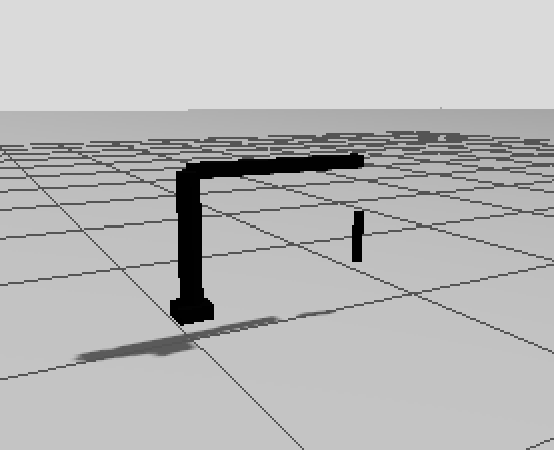
\includegraphics[width=0.75\textwidth]{screenshots/gazebo.png}
    \caption{SCARA robot spawned in Gazebo Harmonic (ROS2 Jazzy). The base column,
             two horizontal arm links, and the vertical prismatic end-effector shaft
             are visible.}
    \label{fig:gazebo}
\end{figure}

\subsection{URDF Definition}

The robot was defined in \texttt{scara.urdf}. Key structural elements are shown
below. The full file is included with the submission.

\begin{lstlisting}[style=ros, language=XML, caption={URDF joint definitions (excerpt)}]
<!-- Joint 1: revolute about z -->
<joint name="joint_1" type="revolute">
    <parent link="base_link"/>
    <child link="link_1"/>
    <origin xyz="0 0 0.05"/>
    <axis xyz="0 0 1"/>
    <limit effort="1000" lower="-1.57" upper="1.57" velocity="0.5"/>
</joint>

<!-- Joint 2: revolute about z -->
<joint name="joint_2" type="revolute">
    <parent link="arm_1"/>
    <child link="link_2"/>
    <origin xyz="0.4 0 0"/>
    <axis xyz="0 0 1"/>
    <limit effort="1000" lower="-1.57" upper="1.57" velocity="0.5"/>
</joint>

<!-- Joint 3: prismatic along z -->
<joint name="joint_3" type="prismatic">
    <parent link="link_2"/>
    <child link="link_3"/>
    <origin xyz="0.3 0 0"/>
    <axis xyz="0 0 1"/>
    <limit effort="1000" lower="-0.2" upper="0.2" velocity="0.5"/>
</joint>
\end{lstlisting}

% ===========================================================================
\section{Forward Kinematics}
% ===========================================================================

\subsection{Mathematical Derivation}

The forward kinematics were derived using the Denavit-Hartenberg (DH) method,
following the convention introduced in lecture. The total transformation from
the base frame to the end-effector frame is:

\[
T_3^0 = T_1^0 \cdot T_2^1 \cdot T_3^2
\]

The resulting closed-form homogeneous transformation matrix is:

\[
T_3^0 =
\begin{bmatrix}
c_{12} & -s_{12} & 0 & -a_2 s_{12} - a_1 s_1 \\
s_{12} &  c_{12} & 0 &  a_2 c_{12} + a_1 c_1 \\
0      &  0      & 1 &  l_1 - d_3 \\
0      &  0      & 0 &  1
\end{bmatrix}
\]

where $c_{12} = \cos(\theta_1 + \theta_2)$, $s_{12} = \sin(\theta_1 + \theta_2)$,
$c_1 = \cos\theta_1$, and $s_1 = \sin\theta_1$.

The end-effector position is therefore:
\begin{align}
p_x &= -a_2 s_{12} - a_1 s_1 \\
p_y &= \phantom{-}a_2 c_{12} + a_1 c_1 \\
p_z &= l_1 - d_3
\end{align}

\subsection{ROS2 Node Implementation}

A ROS2 Python node (\texttt{fk\_node.py}) was implemented in the
\texttt{scara\_fk} package. The node:

\begin{enumerate}
    \item Subscribes to \texttt{/joint\_states} (published by Gazebo)
    \item Computes the end-effector pose using the closed-form FK above
    \item Publishes the result as a \texttt{geometry\_msgs/msg/Pose} message
          on \texttt{/scara/ee\_pose}
\end{enumerate}

\begin{lstlisting}[style=ros, language=Python, caption={FK computation (fk\_node.py excerpt)}]
def joint_state_callback(self, msg: JointState):
    theta1 = self._get_joint(msg, 'joint_1')
    theta2 = self._get_joint(msg, 'joint_2')
    d3     = self._get_joint(msg, 'joint_3')

    c1  = math.cos(theta1);  s1  = math.sin(theta1)
    c12 = math.cos(theta1 + theta2)
    s12 = math.sin(theta1 + theta2)

    px = -A2 * s12 - A1 * s1   # A1=0.40, A2=0.30
    py =  A2 * c12 + A1 * c1
    pz =  L1 - d3               # L1=0.45

    # Pure rotation about z by (theta1 + theta2) -> quaternion
    half = (theta1 + theta2) / 2.0
    pose.orientation.z = math.sin(half)
    pose.orientation.w = math.cos(half)
    self.pub.publish(pose)
\end{lstlisting}

\subsection{Result}

The node was run while the robot was at its default joint configuration
($\theta_1 = 0$, $\theta_2 = 0$, $d_3 = -0.2$ m). The expected end-effector
position is:
\[
p = \bigl(-0.0,\; a_1 + a_2,\; l_1 - d_3\bigr)
  = \bigl(0,\; 0.7,\; 0.65\bigr) \text{ m}
\]

This matches the terminal output shown below.

\begin{figure}[H]
    \centering
    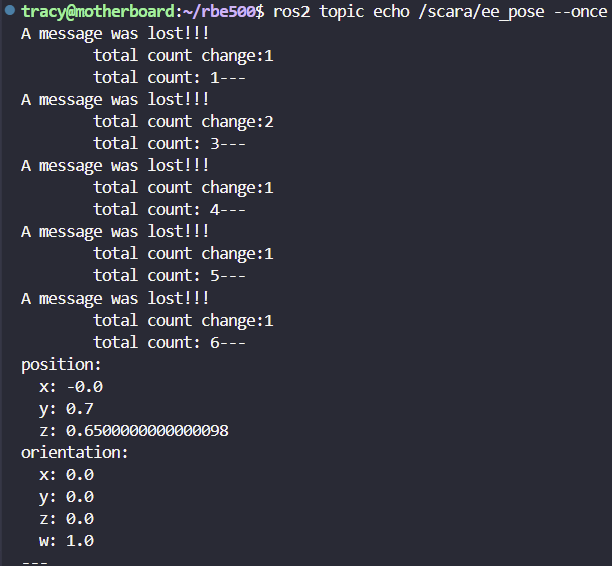
\includegraphics[width=0.85\textwidth]{screenshots/fk_echo.png}
    \caption{Terminal output of \texttt{ros2 topic echo /scara/ee\_pose --once}.
             Position $(x, y, z) = (-0.0,\; 0.7,\; 0.65)$ m and identity
             orientation (all joints at zero) are reported correctly.}
    \label{fig:fk}
\end{figure}

% ===========================================================================
\section{Inverse Kinematics}
% ===========================================================================

\subsection{Mathematical Derivation}

The inverse kinematics problem solves for joint values $(\theta_1, \theta_2, d_3)$
given a desired end-effector position $(p_x, p_y, p_z)$.

\textbf{Step 1 --- $d_3$ directly from $p_z$:}
\[
d_3 = l_1 - p_z
\]

\textbf{Step 2 --- $\theta_2$ via the law of cosines:}
\[
r^2 = p_x^2 + p_y^2, \qquad
\cos\theta_2 = \frac{r^2 - a_1^2 - a_2^2}{2 a_1 a_2}
\]
\[
\theta_2 = \text{atan2}\!\left(+\sqrt{1 - \cos^2\theta_2},\; \cos\theta_2\right)
\quad \text{(elbow-up solution)}
\]

\textbf{Step 3 --- $\theta_1$ algebraically:}

Defining $k_1 = a_1 + a_2\cos\theta_2$ and $k_2 = a_2\sin\theta_2$, and
substituting into the FK position equations yields the $2\times2$ linear system:
\[
\theta_1 = \text{atan2}\!\left(-p_x k_1 - p_y k_2,\;\; p_y k_1 - p_x k_2\right)
\]

\subsection{ROS2 Node Implementation}

A ROS2 Python node (\texttt{ik\_node.py}) was implemented in the
\texttt{scara\_ik\_node} package. The node creates a service at
\texttt{/scara/compute\_ik} using a custom service type
\texttt{scara\_ik/srv/ScaraIK}:

\begin{lstlisting}[style=ros, caption={ScaraIK.srv service definition}]
# Request: desired end-effector position
float64 x
float64 y
float64 z
---
# Response: joint values and success flag
float64 theta1
float64 theta2
float64 d3
bool success
string message
\end{lstlisting}

\begin{lstlisting}[style=ros, language=Python, caption={IK solver (ik\_node.py excerpt)}]
def ik_callback(self, request, response):
    px, py, pz = request.x, request.y, request.z

    # Step 1: d3
    d3 = L1 - pz

    # Step 2: theta2
    r_sq = px**2 + py**2
    c2   = (r_sq - A1**2 - A2**2) / (2.0 * A1 * A2)
    s2   = math.sqrt(1.0 - c2**2)          # elbow-up
    theta2 = math.atan2(s2, c2)

    # Step 3: theta1
    k1 = A1 + A2 * c2
    k2 = A2 * s2
    theta1 = math.atan2(-px*k1 - py*k2,
                         py*k1 - px*k2)

    response.theta1  = theta1
    response.theta2  = theta2
    response.d3      = d3
    response.success = True
    return response
\end{lstlisting}

\subsection{Result}

The IK service was tested with the \texttt{ros2 service call} command for the
target position $(x, y, z) = (0.35, 0.45, 0.25)$ m.

\begin{figure}[H]
    \centering
    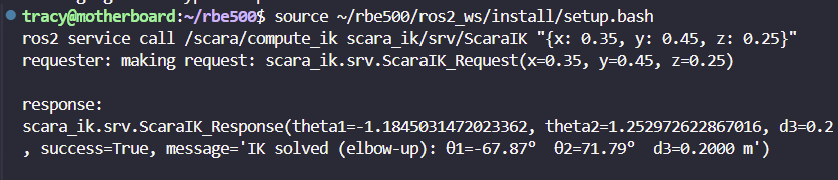
\includegraphics[width=0.9\textwidth]{screenshots/ik_service.png}
    \caption{Terminal output of the \texttt{ros2 service call} command.
             The IK solver returns $\theta_1 = -67.87^{\circ}$, $\theta_2 = 71.79^{\circ}$,
             $d_3 = 0.2$ m with \texttt{success=True}.}
    \label{fig:ik}
\end{figure}

\subsection{Verification}

The solution can be verified by substituting back into the FK equations:
\begin{align*}
\theta_1 &= -67.87^{\circ} = -1.1845 \text{ rad}, \quad
\theta_2 = 71.79^{\circ} = 1.2530 \text{ rad}, \quad d_3 = 0.2 \text{ m} \\[4pt]
p_x &= -0.30\,\sin(-67.87^{\circ} + 71.79^{\circ}) - 0.40\,\sin(-67.87^{\circ}) \approx 0.35 \quad \checkmark \\
p_y &= \phantom{-}0.30\,\cos(-67.87^{\circ} + 71.79^{\circ}) + 0.40\,\cos(-67.87^{\circ}) \approx 0.45 \quad \checkmark \\
p_z &= 0.45 - 0.2 = 0.25 \quad \checkmark
\end{align*}

% ===========================================================================
\section{Package Structure}
% ===========================================================================

The submission includes three ROS2 packages inside \texttt{ros2\_ws/src/}:

\begin{itemize}
    \item \texttt{scara\_description} --- URDF, launch file, and Gazebo configuration
    \item \texttt{scara\_fk} --- Forward kinematics node (Python, \texttt{ament\_python})
    \item \texttt{scara\_ik} --- Custom \texttt{ScaraIK} service definition (\texttt{ament\_cmake})
    \item \texttt{scara\_ik\_node} --- Inverse kinematics service node (Python, \texttt{ament\_python})
\end{itemize}

\end{document}